\section{Experiments}
\label{sec:experiments}

% MANUSCRIPT-NODE: EXP-P01
We use two primary controlled environments and two external families. C-U1 is a nonlinear state-conditioned Gaussian environment with six-dimensional numerical contexts, two-dimensional actions, a known state-dependent optimum, and independently sampled train and test contexts from the same distribution. It supports matched quality--distance probes, near/far intervention, and mean--support terminal audits. D-U1 is a shared-network categorical environment with unordered semantic actions and a known reward structure; it supports matched quality--rarity probes, common/rare intervention, and probability-boundary audits. We report C-U1 using the precise term held-out-context or unseen-state generalization. Hopper/D4RL adds a learned critic and long-horizon continuous control, while Countdown adds shared Transformer parameters and sequence-level verification. External tasks establish relevance; controlled environments establish source and causality.

\begin{table*}[t]
\centering
\caption{Evidence roles are separated by design. Controlled environments identify source and causality; external environments establish relevance and task effect.}
\label{tab:environment_roles}
\small
\begin{tabular}{p{0.14\textwidth}p{0.38\textwidth}p{0.38\textwidth}}
\toprule
Environment & Primary responsibility & Complementary boundary \\
\midrule
C-U1 & Continuous matched source isolation, near/far causality, and phase transition & External relevance is established in Hopper/D4RL; categorical boundaries are tested in D-U1 \\
D-U1 & Categorical matched rarity isolation, common/rare causality, and probability boundary & Gaussian score-amplitude dynamics are tested in C-U1 \\
Hopper/D4RL & External continuous-control occurrence and task effect with a learned critic & Exact badness--distance isolation is supplied by C-U1 \\
Countdown & External shared-parameter sequence occurrence and task effect & Controlled common/rare causality is supplied by D-U1 \\
\bottomrule
\end{tabular}
\end{table*}

% END-MANUSCRIPT-NODE: EXP-P01

% MANUSCRIPT-NODE: EXP-P02
\paragraph{Hopper/D4RL.} We train the registered learned critic, freeze its selected checkpoint, and audit negative actor gradients by current-policy distance. The formal report will include far/near negative-gradient ratios, positive/negative imbalance, policy drift, rollout return, and terminal classification. \textbf{TBD:} insert only terminal-audited formal results from the registered E7 package.

\paragraph{Countdown.} We bin negative tokens or completions by current-policy surprisal and track score magnitude, shared-parameter gradient influence, target-probability change, verifier success, validity, and pass@$k$. \textbf{TBD:} insert only the registered formal result; focused pilots remain provenance rather than final evidence.
% END-MANUSCRIPT-NODE: EXP-P02

% MANUSCRIPT-NODE: EXP-P03
The source-isolation protocol holds sample badness fixed. In C-U1, negative actions share the same state, reward, advantage magnitude, quality coordinate, count, coefficient, and policy parameters while varying only learner-relative radius. We report output-space score norms, full-parameter per-sample gradients, aggregate gradients, and directional coherence. In D-U1, common and rare actions are matched in semantic role, reward, negative advantage, count, and base coefficient while initial probability or current surprisal changes. A far/near or rare/common gap under these controls identifies policy remoteness as an independent amplifier; it does not imply that distance is the only factor in real data.
% END-MANUSCRIPT-NODE: EXP-P03
\begin{figure*}[t]
\centering
\begin{subfigure}{0.48\textwidth}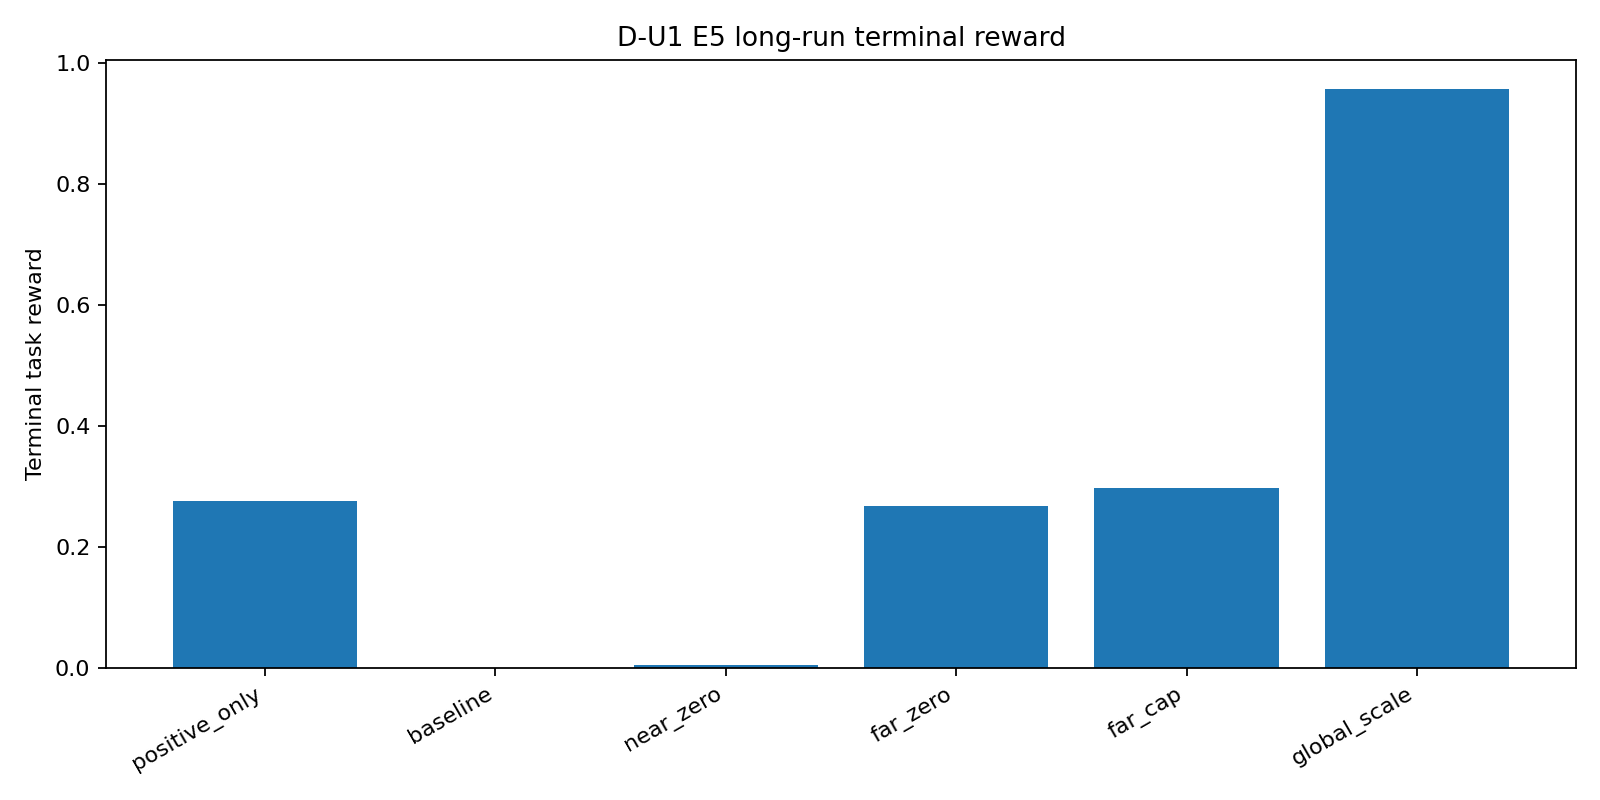
\includegraphics[width=\linewidth]{figures/generated/causal_terminal_reward.png}\caption{Terminal reward.}\end{subfigure}\hfill
\begin{subfigure}{0.48\textwidth}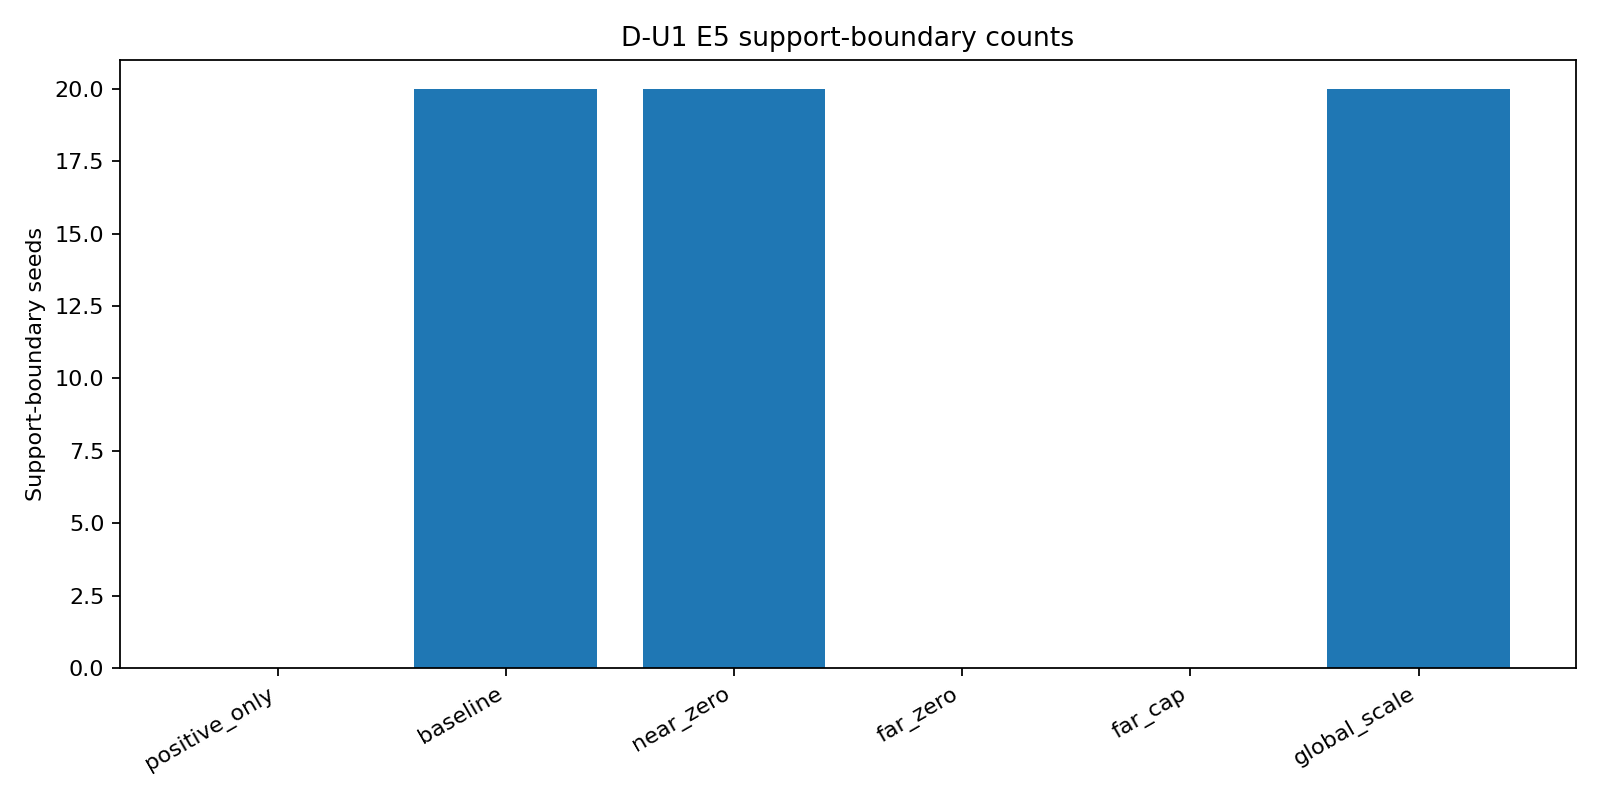
\includegraphics[width=\linewidth]{figures/generated/causal_support_boundary.png}\caption{Support-boundary events.}\end{subfigure}
\caption{D-U1 long-run causal results. Baseline and Near-zero preserve the rare/far negative pathway and reach the support boundary in 20/20 seeds; Far-zero and Far-cap remain bounded in 20/20 seeds. Global scaling can preserve task reward while still reaching the support boundary, illustrating why task, boundary, and numerical events must be reported separately.}
\label{fig:du1-causal}
\end{figure*}
\begin{table}[t]
\centering\small
\caption{D-U1 E5 long-run summary.}
\label{tab:du1-e5}
\begin{tabular}{lccc}
\toprule Method & Reward & Task collapse & Boundary \\
\midrule
baseline & 0.001 & 20/20 & 20/20 \\
near-zero & 0.006 & 20/20 & 20/20 \\
far-zero & 0.267 & 0/20 & 0/20 \\
far-cap & 0.297 & 0/20 & 0/20 \\
global-scale & 0.957 & 0/20 & 20/20 \\
positive-only & 0.275 & 0/20 & 0/20 \\
\bottomrule
\end{tabular}
\end{table}


% MANUSCRIPT-NODE: EXP-P04
We next intervene on the location of negative influence. The continuous comparison includes the uncontrolled signed baseline, Near-zero, Far-zero, Far-cap, a non-selective global control matched to the retained raw negative-gradient budget, and a registered budget-transfer control. The categorical analogue suppresses common or rare negatives under matched counts and budgets. We record the onset order of remote influence, parameter drift, support or probability boundaries, and task performance. A selective far/rare rescue together with an ineffective near/common removal supports the remote component as a causal transmission pathway; task-performance collapse, boundary events, and NaN/Inf remain distinct labels.
% END-MANUSCRIPT-NODE: EXP-P04
\begin{figure*}[t]
\centering
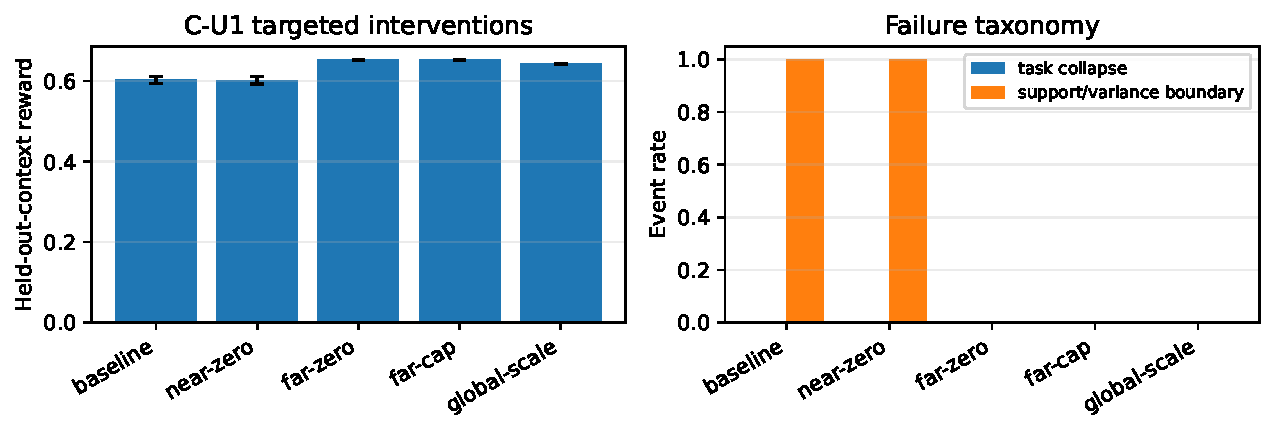
\includegraphics[width=0.93\textwidth]{figures/generated/fig3_cu1_causal.pdf}
\caption{C-U1 causal intervention with learnable variance. The left panel reports registered held-out-context reward with confidence intervals; the right panel separates task-performance collapse from support or variance-boundary events. Near-zero tracks the uncontrolled baseline, while Far-zero and Far-cap remove the task-collapse pathway without introducing NaN/Inf failures.}
\label{fig:cu1-causal}
\end{figure*}
\begin{table}[t]
\centering\small
\caption{C-U1 intervention summary (20 seeds).}
\label{tab:cu1-causal}
\begin{tabular}{lccc}
\toprule Method & Reward & Task event & Boundary event \\
\midrule
baseline & 0.603 & 0.00 & 1.00 \\
near-zero & 0.602 & 0.00 & 1.00 \\
far-zero & 0.653 & 0.00 & 0.00 \\
far-cap & 0.653 & 0.00 & 0.00 \\
global-scale & 0.643 & 0.00 & 0.00 \\
\bottomrule
\end{tabular}
\end{table}


% MANUSCRIPT-NODE: EXP-P05
We sweep the effective negative strength from zero through controlled repulsion and into the unstable regime. The primary test is not a single endpoint score but the phase sequence predicted by Theorem~\ref{thm:equilibrium}: Positive-only, stable extrapolation, boundary approach, and persistent drift or loss of finite equilibrium. We measure a family-specific empirical proxy for the aggregate negative term in~\eqref{eq:weighted-negative-moment}, together with its distance or rarity bins, direction, and relationship to equilibrium displacement. DRPO is compared with Positive-only, global scaling, and registered distance controls under paired seeds and explicit raw-gradient budgets. Results are reported at both selected and terminal checkpoints. \textbf{TBD:} populate the final table only from the current terminal-audited repository artifacts and preserve each result's formal status.

\begin{table*}[t]
\centering
\caption{Controlled phase and method results. Entries remain TBD until the corresponding registered artifacts and terminal audits are frozen for the manuscript. Task collapse, boundary events, and numerical failure are reported separately.}
\label{tab:controlled_results}
\small
\begin{tabular}{lcccccc}
\toprule
Method & Held-out-context reward & Near retention & Far retention & Task collapse & Boundary event & NaN/Inf \\
\midrule
Positive-only & TBD & -- & 0 & TBD & TBD & TBD \\
Uncontrolled signed & TBD & TBD & TBD & TBD & TBD & TBD \\
Global matched & TBD & TBD & TBD & TBD & TBD & TBD \\
Hard distance control & TBD & TBD & TBD & TBD & TBD & TBD \\
DRPO exponential & TBD & TBD & TBD & TBD & TBD & TBD \\
\bottomrule
\end{tabular}
\end{table*}

% END-MANUSCRIPT-NODE: EXP-P05
\begin{figure*}[t]
\centering
\begin{subfigure}{0.62\textwidth}
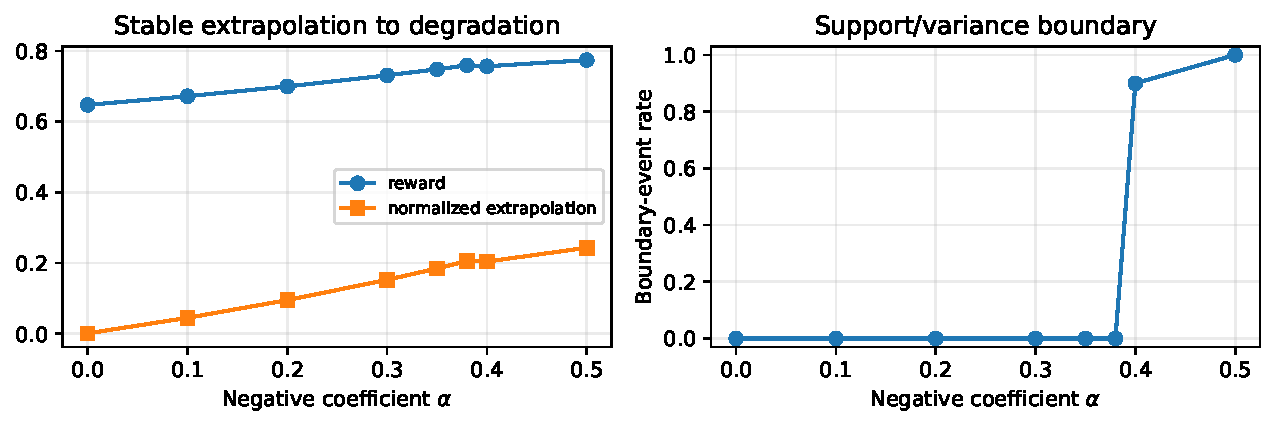
\includegraphics[width=\linewidth]{figures/generated/fig4_cu1_phase.pdf}
\caption{Strength sweep and boundary events.}
\end{subfigure}\hfill
\begin{subfigure}{0.34\textwidth}
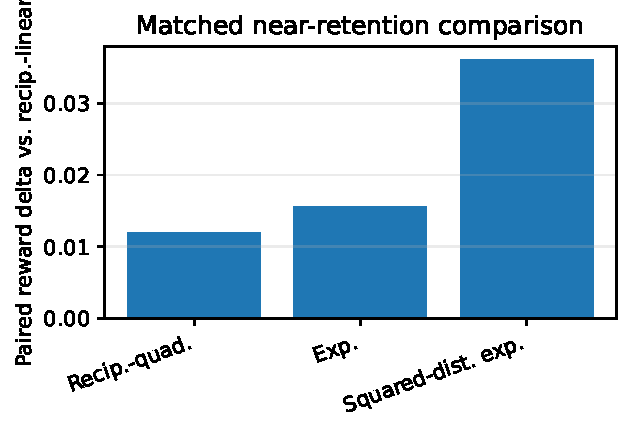
\includegraphics[width=\linewidth]{figures/generated/fig5_taper_shape.pdf}
\caption{Matched near-retention taper comparison.}
\end{subfigure}
\caption{C-U1 phase and control evidence. The strength sweep maps the transition from the Positive-only reference through stable extrapolation toward boundary events. Under the frozen near-retention protocol, all three faster-decaying tapers improve finite-horizon held-out-context reward on 20/20 paired seeds relative to reciprocal-linear; this result remains finite-step validated rather than a universal steady-state ranking.}
\label{fig:cu1-phase-control}
\end{figure*}


% MANUSCRIPT-NODE: EXP-P06
The final evaluation returns to external tasks. On D4RL locomotion, methods share dataset, critic protocol, initialization, seeds, evaluation horizon, and selection rule; we report normalized return, uncertainty, best and terminal checkpoints, and distance-binned negative influence. On Countdown, methods share the SFT initialization, rollout or replay bank, verifier, seeds, and checkpoint-selection protocol; we report greedy success, pass@$k$, validity, terminal degradation, and rare-negative diagnostics. \textbf{TBD:} the main external tables remain unfilled until the corresponding registered formal experiments are terminal-audited and delivered.

\begin{table*}[t]
\centering
\caption{External task closure. Best and terminal results are both required; no values are inserted before formal terminal-audited completion.}
\label{tab:external_results}
\small
\begin{tabular}{llccccc}
\toprule
Family & Dataset/model & Uncontrolled & Positive-only & Global & DRPO & Terminal failure rate \\
\midrule
D4RL & Hopper / locomotion suite & TBD & TBD & TBD & TBD & TBD \\
Countdown & Main model scale & TBD & TBD & TBD & TBD & TBD \\
\bottomrule
\end{tabular}
\end{table*}

% END-MANUSCRIPT-NODE: EXP-P06
